% Apêndices
\begin{apendicesenv}

\partapendices

\chapter{Discussões sobre a verticalização}
\label{appendix:verticalizacao}

Assumindo prédios como paralelepípedos, ou seja, todos os andares apresentam a mesma metragem, é possível traçar relações geométricas nas quais a área ocupada é a superfície que representa a base do paralelepípedo, o número de pavimentos sua altura e a área construída seu volume (Figura \ref{fig:desenho}). Nesse sentido, as relações apresentadas na Equação \ref{eq:pavimentos}, que apresenta diferentes formas de calcular a verticalização, ficam mais claras. Na equação, AC representa a área construída; AO, a área o cupada; AT, a área do terreno; CA o coeficiente de aproveitamento e tx\_ocupacao, o percentual da área do terreno que é ocupada. Usando o procedimento apresentado, em regiões que possuem o mesmo CA, quanto menor for a taxa de ocupação do terreno, maior será a verticalização. Analogamente, para dois lotes com a mesma ocupação de terreno, quanto maior for o CA, maior é a verticalização.

\begin{figure}[h]
    \centering
    \caption{Representação do prédio como um paralelepípedo}
    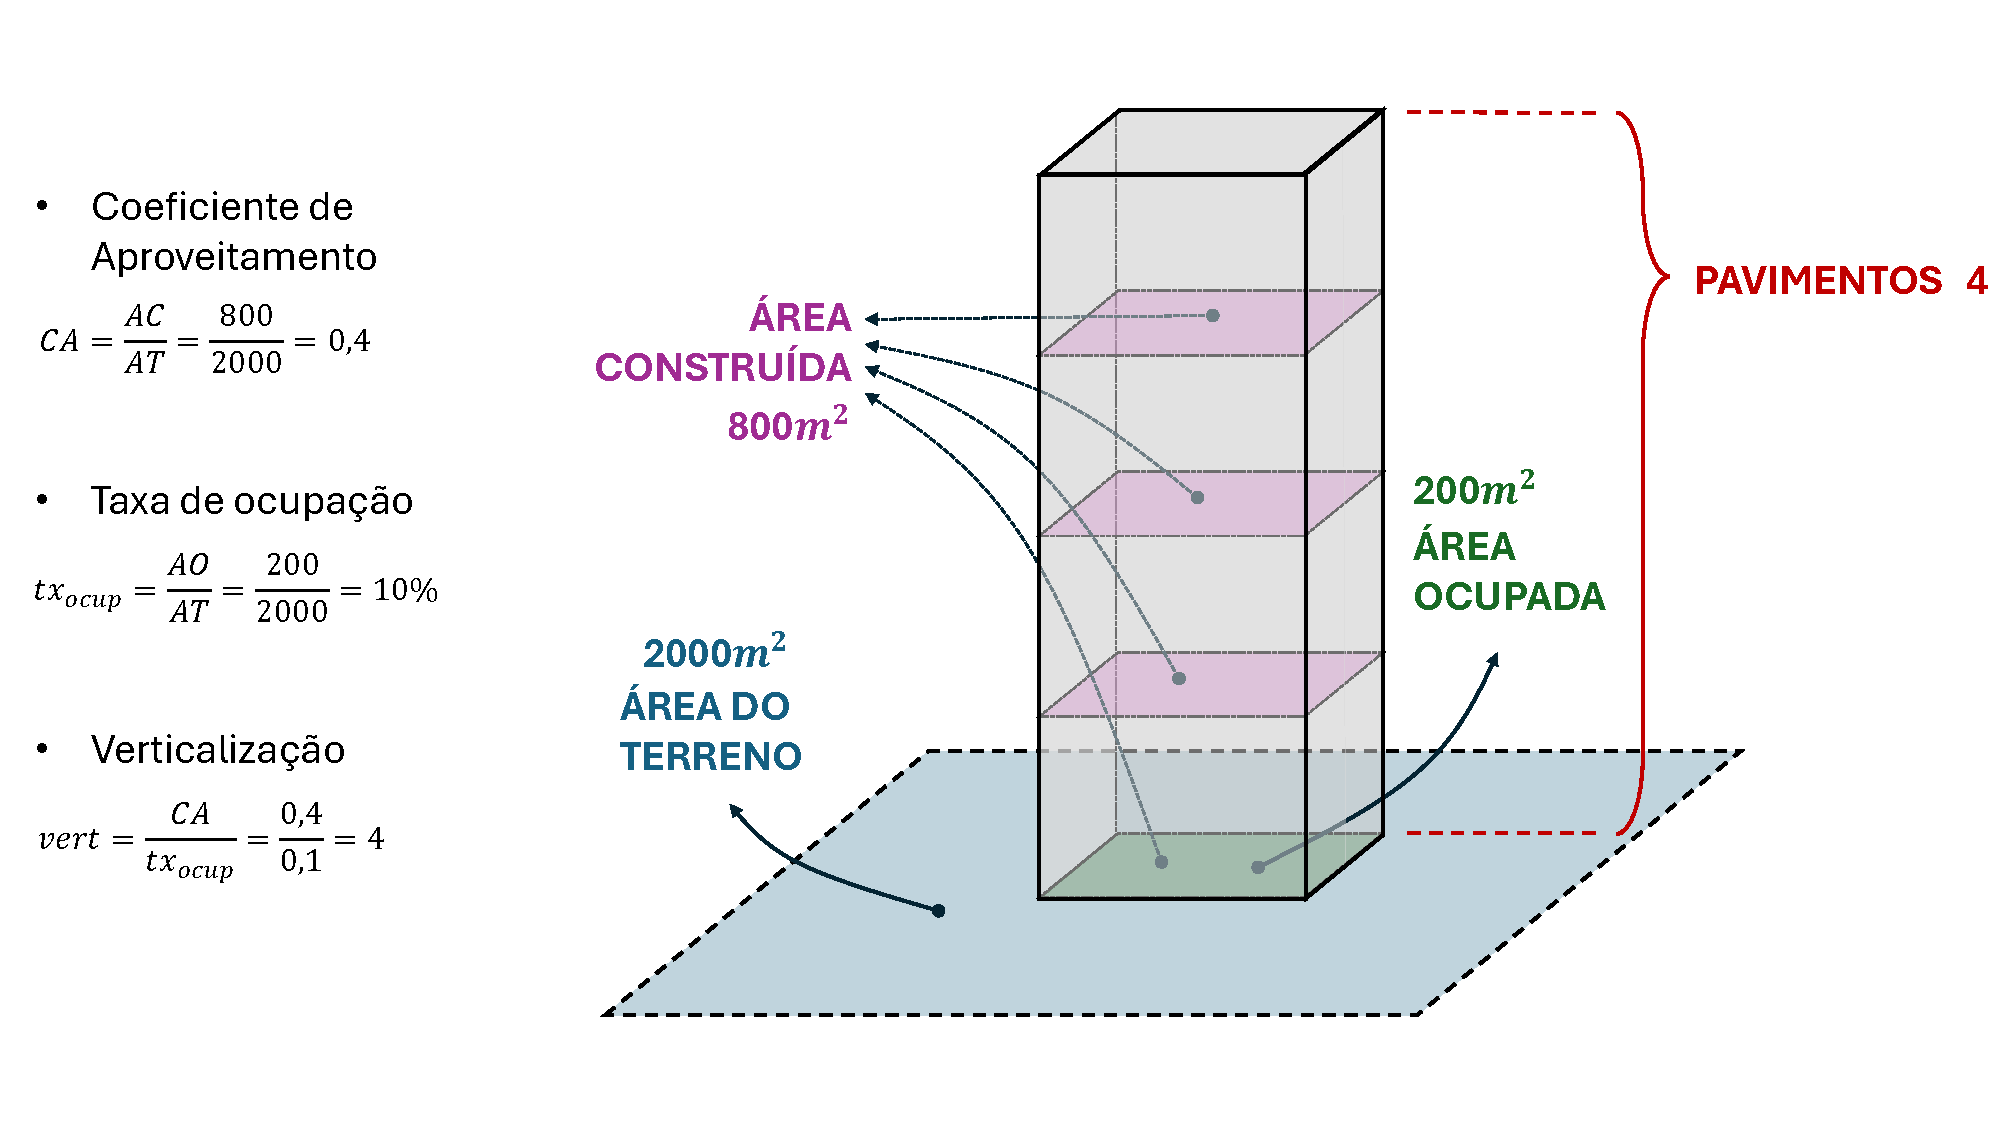
\includegraphics[width = \linewidth]{imagens/desenho.pdf}
    \label{fig:desenho}
\end{figure}

\begin{equation}
    \text{Pavimentos}=\frac{\text{AC}}{\text{AO}}=\frac{\text{AC}}{\text{AT}\cdot\underbrace{\frac{\text{AO}}{\text{AT}}}_\text{tx\_ocup}}=\frac{\text{AC}}{\text{AT}}\div\frac{\text{AO}}{\text{AT}}=\frac{\text{CA}}{\text{tx\_ocup}}
    \label{eq:pavimentos}
\end{equation}
    
Dessa forma, o número de pavimentos nunca será maior do que o CA, dado que a taxa de ocupação sempre é um número que varia entre zero e um. Na Figura \ref{fig:ca-vert} é possível observar a relação entre as duas variáveis. Para lotes muito pequenos, as duas medidas geralmente são iguais, visto que geralmente se ocupa 100\% da área do terreno. Na medida em que a verticalização aumenta, é observável que o CA não acompanha este crescimento, o que indica que há uma queda na taxa de ocupação.

\begin{figure}
    \centering
    \caption{Relação entre densidade construtiva e verticalização}
    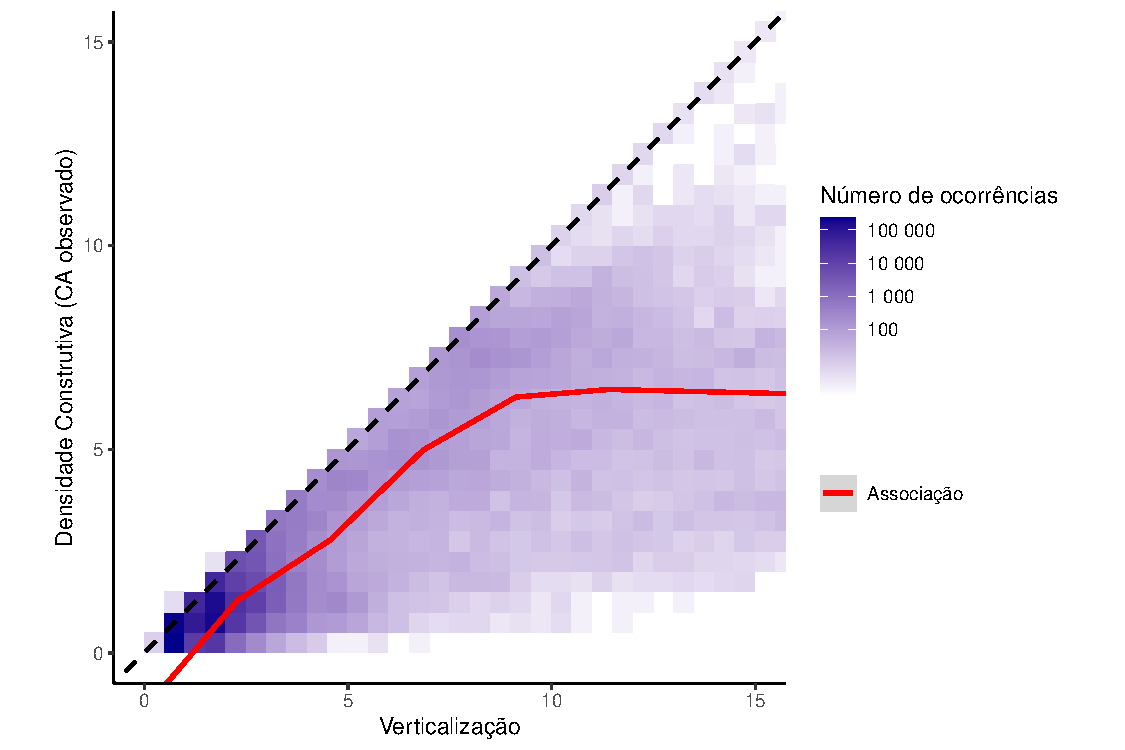
\includegraphics[width = \textwidth]{imagens/ca_vs_verticalizacao.pdf}
    \label{fig:ca-vert}
\end{figure}

\chapter{Rasters de densidade residencial}
\label{appendix:rasters-corte}

A densidade total pode ser calculada utilizando exclusivamente os dados do Censo, enquanto a densidade residencial necessita dos dados do IPTU para calcular a área do terreno. Dessa forma, na medida em que há mais moradia informal, o valor da densidade residencial passa a ser viesado de forma a ser superestimado, visto que a população não muda, mas a área de terreno é subestimada. Na Figura \ref{fig:rasters-dens} é possível observar as células que são removidas para cada nível de corte do espectro de irregularidade.

\begin{figure}[h]
    \centering
    \caption{Rasters de densidade para cada nível de corte do espectro de irregularidade}
    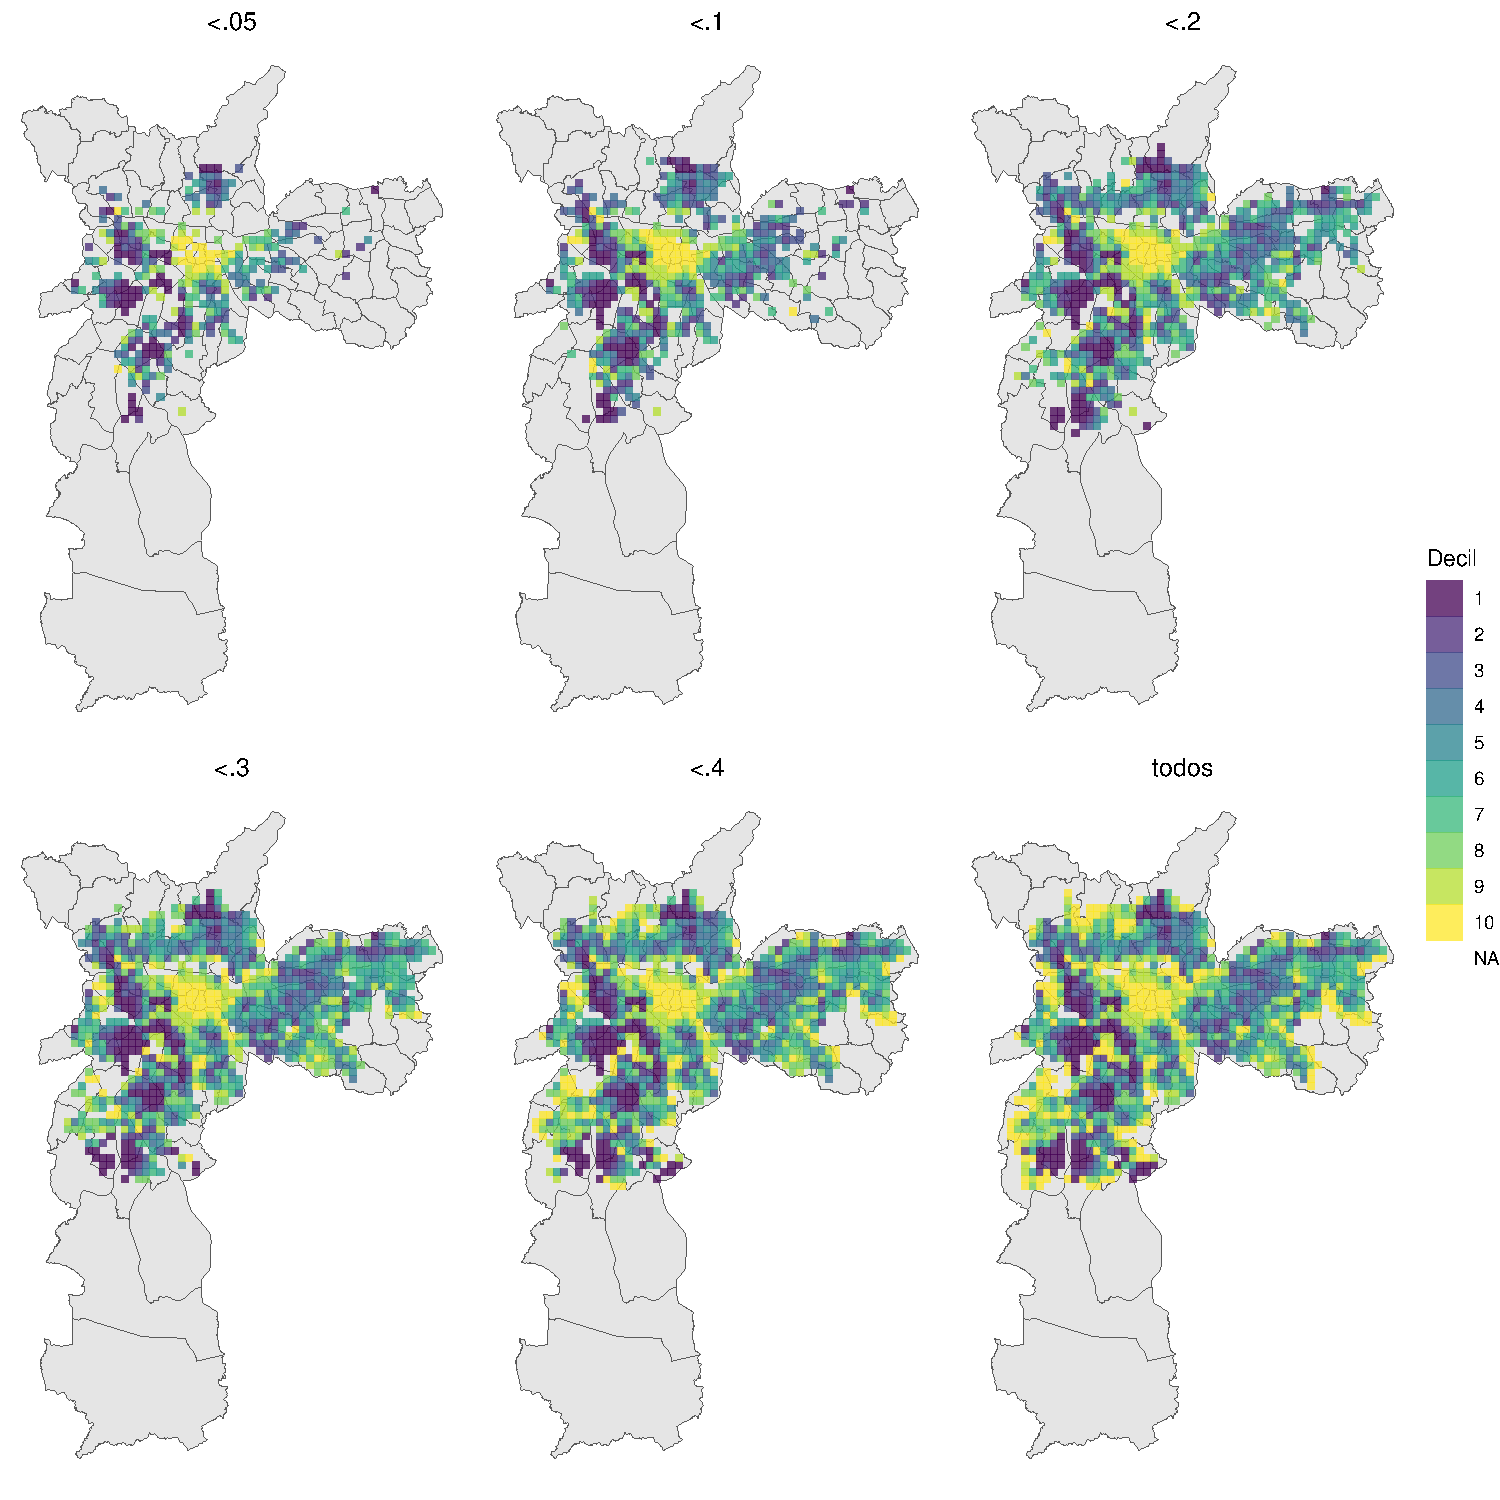
\includegraphics[width = .95\textwidth]{imagens/rasters_densidade.pdf}
    \label{fig:rasters-dens}
\end{figure}




\chapter{Análise de robustez do corte do espectro de irregularidade}
\label{appendix:robustez-corte}

A escolha do corte de espectro de irregularidade é arbitrária, visto que não há um valor que se configure como correto. Dessa forma, os resultados apresentados na Seção \ref{sec:analise} podem alterar na medida em que se escolhe valores diferentes. Na Figura \ref{fig:pvals} é possível observar no eixo x o corte do espectro de irregularidade, ou seja, se este valor é igual a 10\%, o espectro de irregularidade varia entre 40 e 60\%. No eixo y, estão representados os p valores de cada variável explicativa, com a escala em raiz quadrada. Estes valores foram gerados para a regressão com a densidade em nível e em log. Na Figura \ref{fig:nobs} é possível observar o número de observações na medida em que o corte fica mais leniente.

\begin{figure}[h]
    \centering
    \caption{Análise de robustez para corte do espectro de irregularidade}
    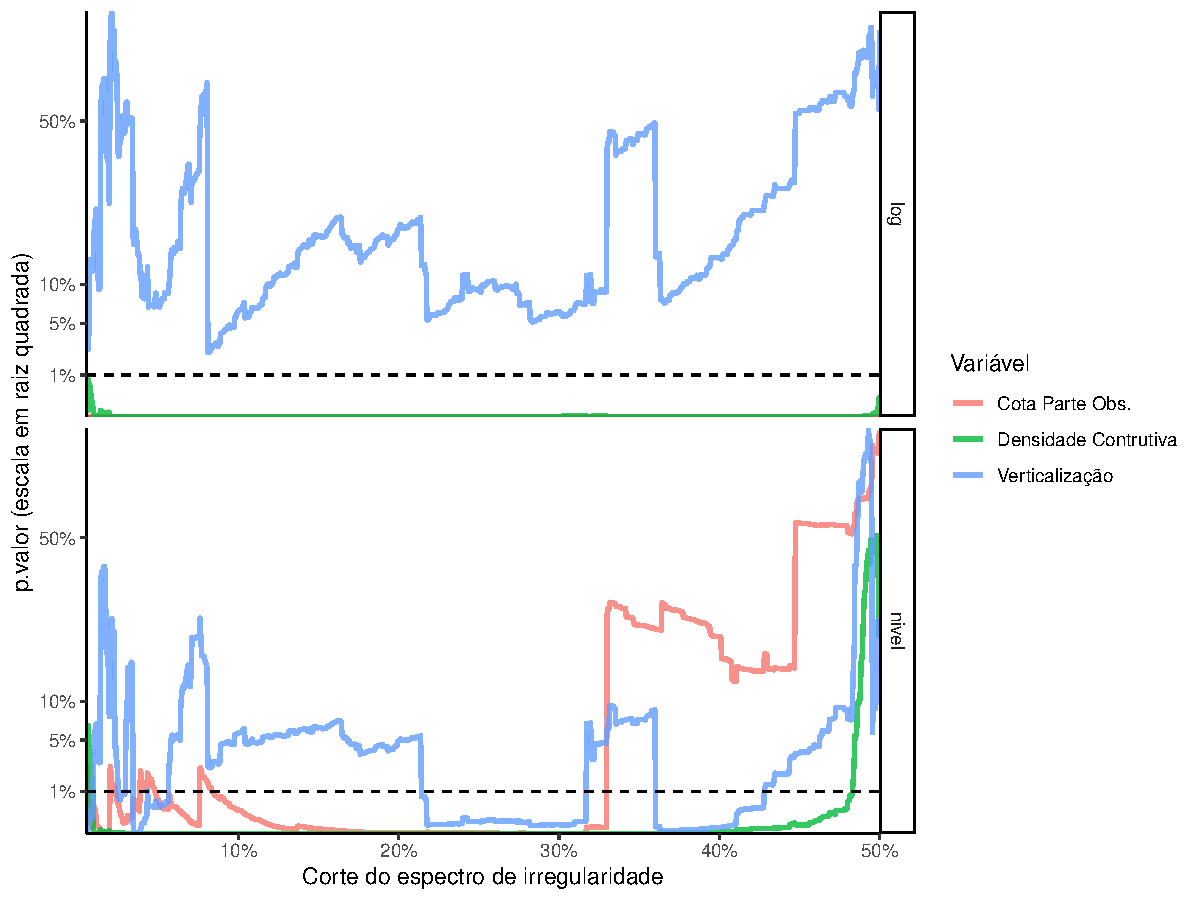
\includegraphics[width = \linewidth]{imagens/pvals.pdf}
    \label{fig:pvals}
\end{figure}

Para a regressão com a densidade em escala logarítmica, não importa a escolha de corte, a verticalização apresenta um p valor sempre maior do que 1\%, mas para alguns níveis ela se mostra relevante a 10\%. Já o CA e cota parte se mantém significativos a 1\% para qualquer corte. Os resultados para a densidade em nível são diferentes para a verticalização, que passa a apresentar significância de 1\% para algumas faixas de corte específicas. Todavia, ainda é possível afirmar que as evidências de importância do instrumento de verticalização são mais fracas do que dos outros instrumentos.

\begin{figure}[h]
    \centering
    \caption{Observações removidas na medida em que se altera o corte do espectro de irregularidade}
    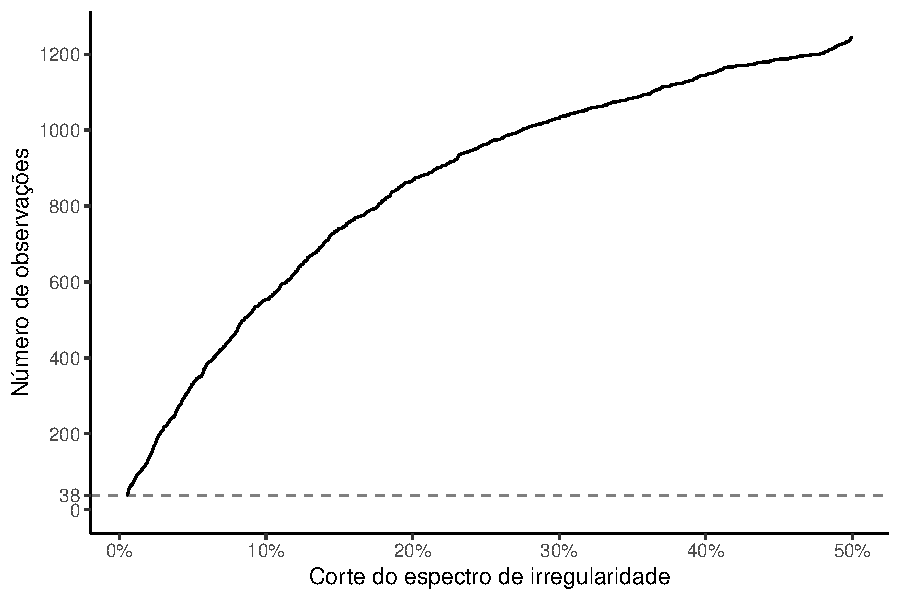
\includegraphics[width = .75\linewidth]{imagens/nobs.pdf}
    \label{fig:nobs}
\end{figure}



\end{apendicesenv}
    
    